\section{Numerical Validations}
\label{sec:numerical_validations}
\subsection{Test Conditions and Evidence}
The saved \texttt{push\_performance\_tables.mat} contains 48 directional response records: six push settings, two plant representations and four controller/sensor cases. These records were checked against the exported performance CSVs. Additional peak-angle, final-angle and simulation-end values are taken from the corresponding per-run CSVs. The experiments compare the linearised and full nonlinear plants using the same nominal 0.737243~kg configuration, 50~Hz state-feedback controller and discrete Luenberger observer. They do not provide a PID comparison.

Each test applies a positive forward ($X$) or sideways ($Y$) torso force
\[
F(t)=F_0\exp\!\left[-\left(\frac{t-0.2}{0.02}\right)^2\right],
\quad F_0\in\{1,5,10\}\ \mathrm{N},
\]
with zero independently applied body moment. These are forces in newtons, not moments in N\,m. Their approximate impulses are 0.0354, 0.1772 and 0.3545~N\,s. Runs request 3~s and terminate early if the model-validity limits are reached. The physical plant starts at standing trim; the observer starts with $0.5^\circ$ roll and $1^\circ$ pitch estimation errors. Consequently, the measured response includes the controller's initial estimation transient as well as the push response.

Cases A--D respectively use: inner servos without outer balance feedback; state feedback with observer; the same controller with constant sensor bias; and constant bias plus sinusoidal sensor error. In C, each gyro channel has $0.05^\circ$/s bias, each accelerometer channel has 0.01~m/s$^2$ bias and each encoder has $0.10^\circ$ bias. D adds sinusoidal errors of $0.05^\circ$/s, 0.01~m/s$^2$ and $0.05^\circ$, respectively, at 10~rad/s. These deterministic errors enter the sampled measurement path, not the external push or motor torque. They do not constitute stochastic white-noise trials. The nonlinear plant retains actuator lag, command/torque limits and contact dynamics; saturation is bypassed in the linear comparison.

\subsection{Transient-Metric Definitions}
The lecture's step-response measures require care because the reference remains upright before and after a push. Let $\alpha$ be actual pitch for forward pushes or roll for sideways pushes, measured relative to trim. The analysis starts at $t_0=0.2-3(0.02)=0.14$~s. Define $A=\max_{t\ge t_0}|\alpha(t)|$, its occurrence time $t^*$, and $s=\operatorname{sign}(\alpha(t^*))$. The reported $t_r$ is the first 10--90\% rise of $s\alpha$ towards $A$, and $t_p=t^*-t_0$. A shorter excursion rise time therefore does not necessarily indicate better disturbance rejection.

Settling time $t_s$ is measured from $t_0$ to the first time after the peak for which $|\alpha|\le0.02A$ throughout the remaining record, with at least 0.5~s of in-band observations and a completed simulation. An absent value means this condition was not established. The reverse-excursion ratio is
\[
M_{\rm rev}=100\frac{\max\{0,-\min_{t\ge t^*}(s\alpha(t))\}}{A}.
\]
It measures the subsequent opposite-side excursion and is not conventional percentage overshoot of a nonzero reference step. Likewise, a zero value does not establish successful regulation. Peaks recorded at an early-stop boundary are truncated excursions, not completed transient peaks. Tables~\ref{tab:push_nonlinear} and~\ref{tab:push_linear} retain these entries and explicitly identify incomplete runs. Their final angles describe the last recorded sample, not a proven steady state.

\begin{table*}[!t]
\centering\footnotesize
\caption{Nonlinear push-response results. Forward tests report pitch; sideways tests report roll. Times are in seconds, angles in degrees, and $M_{\rm rev}$ in percent. A: inner servos only; B: state feedback and observer; C: B with bias; D: C with sinusoidal sensor error. ``--'' means settling was not established, not zero settling time.}
\label{tab:push_nonlinear}
\setlength{\tabcolsep}{5pt}
\begin{tabular}{@{}llcrrrrrrrcc@{}}
\toprule
Direction & $F_0$ (N) & Case & $t_r$ & $t_p$ & $t_s$ & $M_{\rm rev}$ & Peak $|\alpha|$ & Final $\alpha$ & End time & Complete & Settled\\
\midrule
Forward & 1 & A & 0.638 & 0.892 & -- & 0.00 & 19.970 & 19.970 & 1.032 & No & No\\
Forward & 1 & B & 0.111 & 0.302 & 1.267 & 0.00 & 1.474 & 0.000 & 3.000 & Yes & Yes\\
Forward & 1 & C & 0.118 & 0.310 & -- & 0.00 & 1.656 & 0.304 & 3.000 & Yes & No\\
Forward & 1 & D & 0.119 & 0.309 & -- & 0.00 & 1.708 & 0.333 & 3.000 & Yes & No\\
\midrule
Forward & 5 & A & 0.228 & 0.366 & -- & 0.00 & 19.970 & 19.970 & 0.506 & No & No\\
Forward & 5 & B & 0.184 & 0.381 & 1.297 & 0.00 & 10.131 & 0.000 & 3.000 & Yes & Yes\\
Forward & 5 & C & 0.193 & 0.392 & -- & 0.00 & 10.458 & 0.304 & 3.000 & Yes & No\\
Forward & 5 & D & 0.195 & 0.395 & -- & 0.00 & 10.555 & 0.333 & 3.000 & Yes & No\\
\midrule
Forward & 10 & A & 0.096 & 0.210 & -- & 0.00 & 19.970 & 19.970 & 0.350 & No & No\\
Forward & 10 & B & 0.133 & 0.261 & -- & 0.00 & 19.970 & 19.970 & 0.401 & No & No\\
Forward & 10 & C & 0.132 & 0.259 & -- & 0.00 & 19.970 & 19.970 & 0.399 & No & No\\
Forward & 10 & D & 0.131 & 0.258 & -- & 0.00 & 19.970 & 19.970 & 0.398 & No & No\\
\midrule
Sideways & 1 & A & 0.022 & 0.112 & 0.668 & 55.52 & 0.107 & -0.000 & 3.000 & Yes & Yes\\
Sideways & 1 & B & 0.022 & 0.113 & 0.666 & 55.57 & 0.108 & -0.000 & 3.000 & Yes & Yes\\
Sideways & 1 & C & 0.022 & 0.112 & 0.666 & 55.52 & 0.108 & 0.000 & 3.000 & Yes & Yes\\
Sideways & 1 & D & 0.022 & 0.112 & 0.666 & 55.51 & 0.108 & 0.000 & 3.000 & Yes & Yes\\
\midrule
Sideways & 5 & A & 0.041 & 0.161 & -- & 51.53 & 0.852 & -0.002 & 2.188 & No & No\\
Sideways & 5 & B & 0.041 & 0.161 & 0.824 & 51.61 & 0.855 & -0.000 & 3.000 & Yes & Yes\\
Sideways & 5 & C & 0.041 & 0.161 & 0.824 & 51.56 & 0.854 & -0.000 & 3.000 & Yes & Yes\\
Sideways & 5 & D & 0.041 & 0.161 & 0.824 & 51.56 & 0.854 & -0.000 & 3.000 & Yes & Yes\\
\midrule
Sideways & 10 & A & 0.158 & 0.306 & -- & 6.31 & 3.289 & 0.047 & 1.828 & No & No\\
Sideways & 10 & B & 0.124 & 0.314 & 1.098 & 7.23 & 3.195 & -0.000 & 3.000 & Yes & Yes\\
Sideways & 10 & C & 0.127 & 0.309 & 1.094 & 7.14 & 3.189 & -0.000 & 3.000 & Yes & Yes\\
Sideways & 10 & D & 0.128 & 0.307 & 1.095 & 7.14 & 3.187 & -0.000 & 3.000 & Yes & Yes\\
\bottomrule\end{tabular}\end{table*}
\begin{table*}[!t]
\centering\footnotesize
\caption{Linear push-response results. Forward tests report pitch; sideways tests report roll. Times are in seconds, angles in degrees, and $M_{\rm rev}$ in percent. A: inner servos only; B: state feedback and observer; C: B with bias; D: C with sinusoidal sensor error. ``--'' means settling was not established, not zero settling time.}
\label{tab:push_linear}
\setlength{\tabcolsep}{5pt}
\begin{tabular}{@{}llcrrrrrrrcc@{}}
\toprule
Direction & $F_0$ (N) & Case & $t_r$ & $t_p$ & $t_s$ & $M_{\rm rev}$ & Peak $|\alpha|$ & Final $\alpha$ & End time & Complete & Settled\\
\midrule
Forward & 1 & A & 0.639 & 0.893 & -- & 0.00 & 19.970 & 19.970 & 1.033 & No & No\\
Forward & 1 & B & 0.111 & 0.302 & 1.278 & 0.00 & 1.475 & 0.000 & 3.000 & Yes & Yes\\
Forward & 1 & C & 0.118 & 0.310 & -- & 0.00 & 1.657 & 0.304 & 3.000 & Yes & No\\
Forward & 1 & D & 0.119 & 0.309 & -- & 0.00 & 1.710 & 0.334 & 3.000 & Yes & No\\
\midrule
Forward & 5 & A & 0.228 & 0.365 & -- & 0.00 & 19.970 & 19.970 & 0.505 & No & No\\
Forward & 5 & B & 0.121 & 0.288 & 1.266 & 0.00 & 9.212 & 0.000 & 3.000 & Yes & Yes\\
Forward & 5 & C & 0.122 & 0.289 & -- & 0.00 & 9.386 & 0.304 & 3.000 & Yes & No\\
Forward & 5 & D & 0.122 & 0.289 & -- & 0.00 & 9.439 & 0.334 & 3.000 & Yes & No\\
\midrule
Forward & 10 & A & 0.107 & 0.218 & -- & 0.00 & 19.970 & 19.970 & 0.358 & No & No\\
Forward & 10 & B & 0.122 & 0.286 & 1.265 & 0.00 & 18.892 & 0.000 & 3.000 & Yes & Yes\\
Forward & 10 & C & 0.123 & 0.287 & 1.577 & 0.00 & 19.065 & 0.304 & 3.000 & Yes & Yes\\
Forward & 10 & D & 0.123 & 0.287 & 1.647 & 0.00 & 19.117 & 0.334 & 3.000 & Yes & Yes\\
\midrule
Sideways & 1 & A & 0.022 & 0.111 & 0.666 & 55.54 & 0.107 & -0.000 & 3.000 & Yes & Yes\\
Sideways & 1 & B & 0.022 & 0.112 & 0.667 & 55.53 & 0.107 & -0.000 & 3.000 & Yes & Yes\\
Sideways & 1 & C & 0.022 & 0.112 & 0.666 & 55.53 & 0.107 & -0.000 & 3.000 & Yes & Yes\\
Sideways & 1 & D & 0.022 & 0.112 & 0.666 & 55.52 & 0.107 & -0.000 & 3.000 & Yes & Yes\\
\midrule
Sideways & 5 & A & 0.022 & 0.112 & 0.667 & 55.53 & 0.537 & -0.000 & 3.000 & Yes & Yes\\
Sideways & 5 & B & 0.022 & 0.113 & 0.668 & 55.53 & 0.537 & -0.000 & 3.000 & Yes & Yes\\
Sideways & 5 & C & 0.022 & 0.112 & 0.667 & 55.53 & 0.537 & -0.000 & 3.000 & Yes & Yes\\
Sideways & 5 & D & 0.022 & 0.112 & 0.667 & 55.53 & 0.537 & -0.000 & 3.000 & Yes & Yes\\
\midrule
Sideways & 10 & A & 0.022 & 0.112 & 0.667 & 55.52 & 1.074 & -0.000 & 3.000 & Yes & Yes\\
Sideways & 10 & B & 0.022 & 0.112 & 0.666 & 55.53 & 1.074 & -0.000 & 3.000 & Yes & Yes\\
Sideways & 10 & C & 0.022 & 0.112 & 0.666 & 55.53 & 1.074 & -0.000 & 3.000 & Yes & Yes\\
Sideways & 10 & D & 0.022 & 0.112 & 0.666 & 55.53 & 1.074 & -0.000 & 3.000 & Yes & Yes\\
\bottomrule\end{tabular}\end{table*}

\subsection{Forward-Push Recovery and Linear-Model Limits}
For the nonlinear 1~N test, B limits peak pitch to $1.474^\circ$, with $t_r=0.111$~s, $t_p=0.302$~s and $t_s=1.267$~s. Its final pitch deviation is approximately $6.4\times10^{-6}\!{}^\circ$. A instead reaches approximately $20^\circ$ and stops at 1.032~s. At 5~N, B completes the run and returns close to upright, but the peak increases to $10.131^\circ$, with $t_s=1.297$~s. Recovery therefore does not imply compliance with a $5^\circ$ peak-tilt criterion. The 10~N nonlinear test is unsuccessful: B reaches the validity boundary and stops at 0.401~s; C and D stop at 0.399 and 0.398~s. No finite recovery or settling time is established for these runs.

The linear and nonlinear 1~N results agree closely: B gives peak pitches of $1.475^\circ$ and $1.474^\circ$, respectively. Differences increase at 5~N, where the linear peak is $9.212^\circ$ and the nonlinear peak is $10.131^\circ$ (about 10\% larger). At 10~N, the linear B run predicts recovery with an $18.892^\circ$ peak and $t_s=1.265$~s, whereas the nonlinear run stops. Thus local linear recovery does not guarantee recovery of the constrained nonlinear plant at larger excursions. These observations do not isolate a single failure mechanism: changing geometry, contact and command constraints all differ from the local linear approximation.

\begin{figure*}[!t]\centering
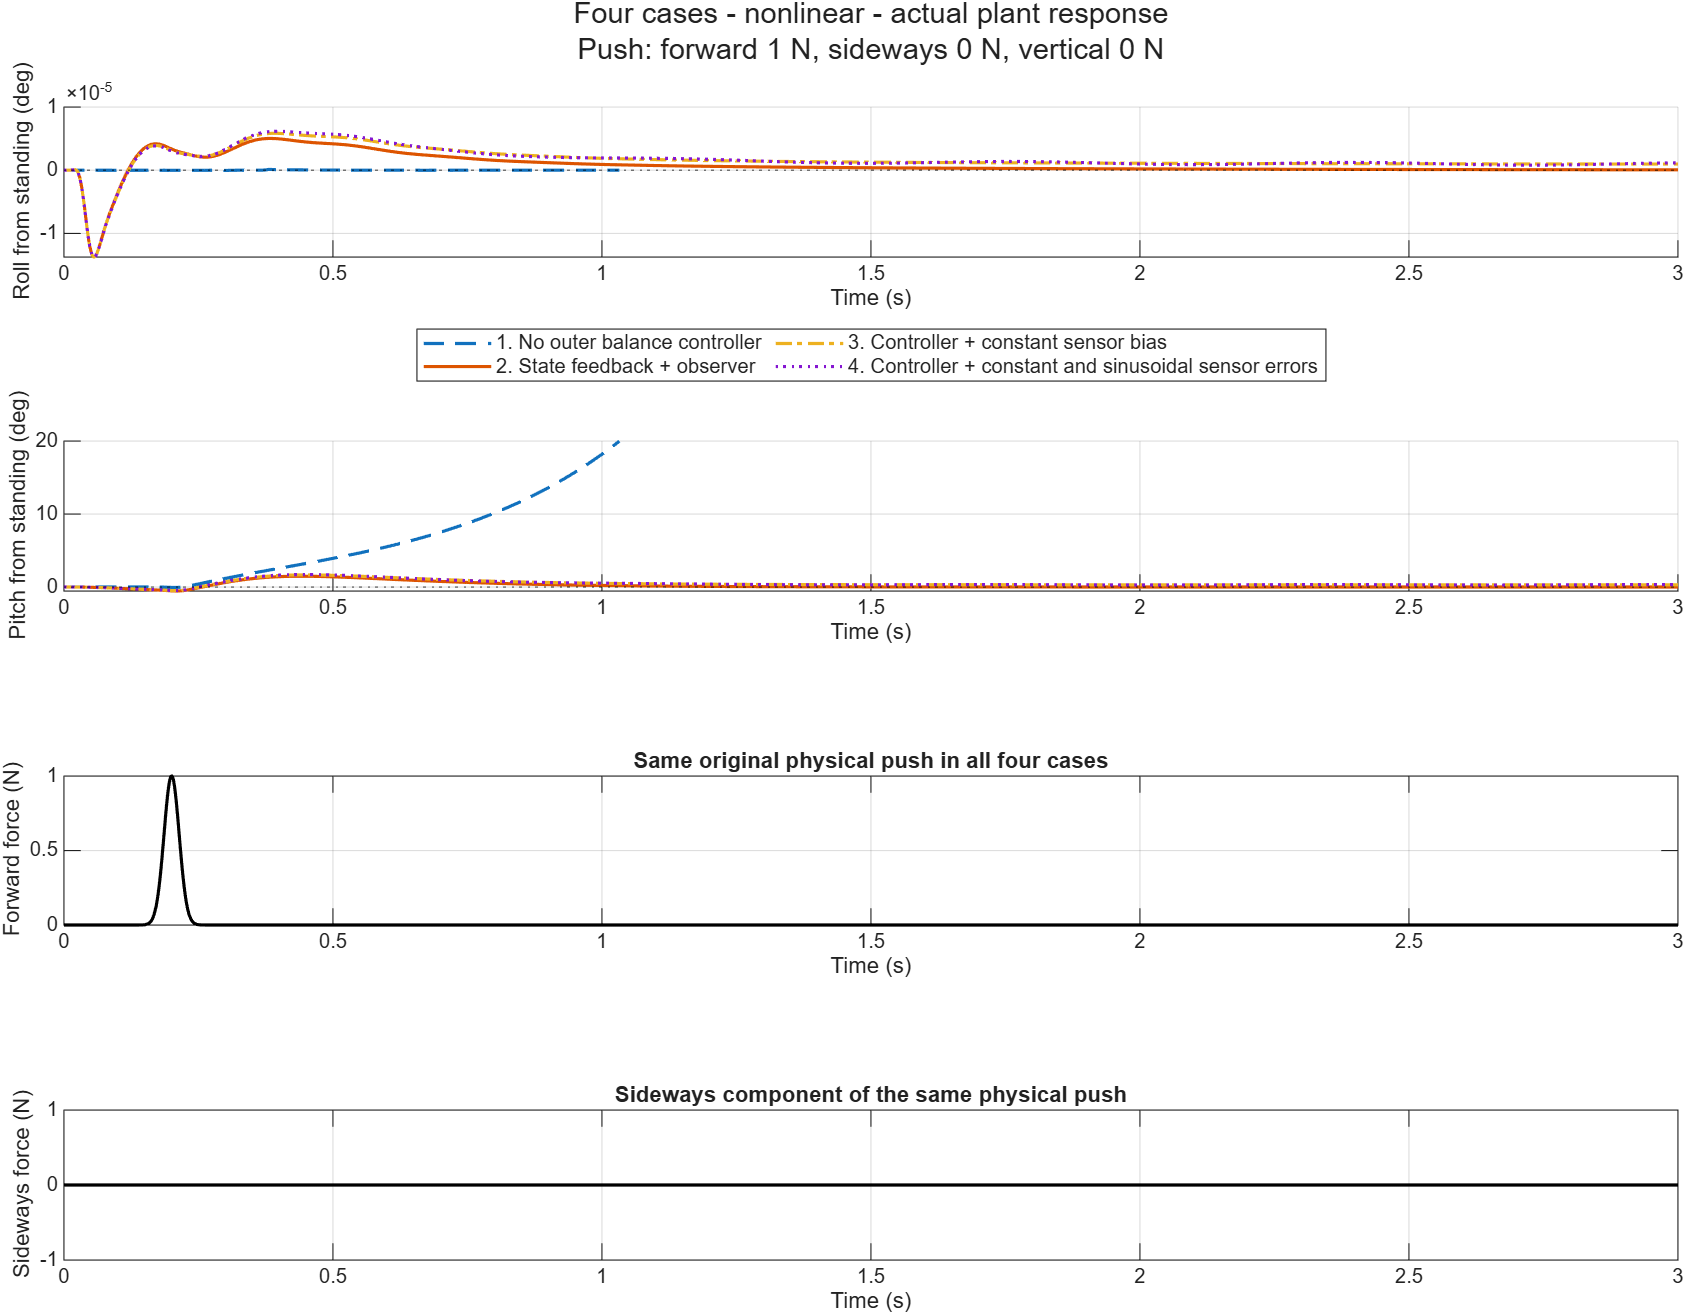
\includegraphics[width=0.485\textwidth]{figures/forward_1N_nonlinear_response.png}\hfill
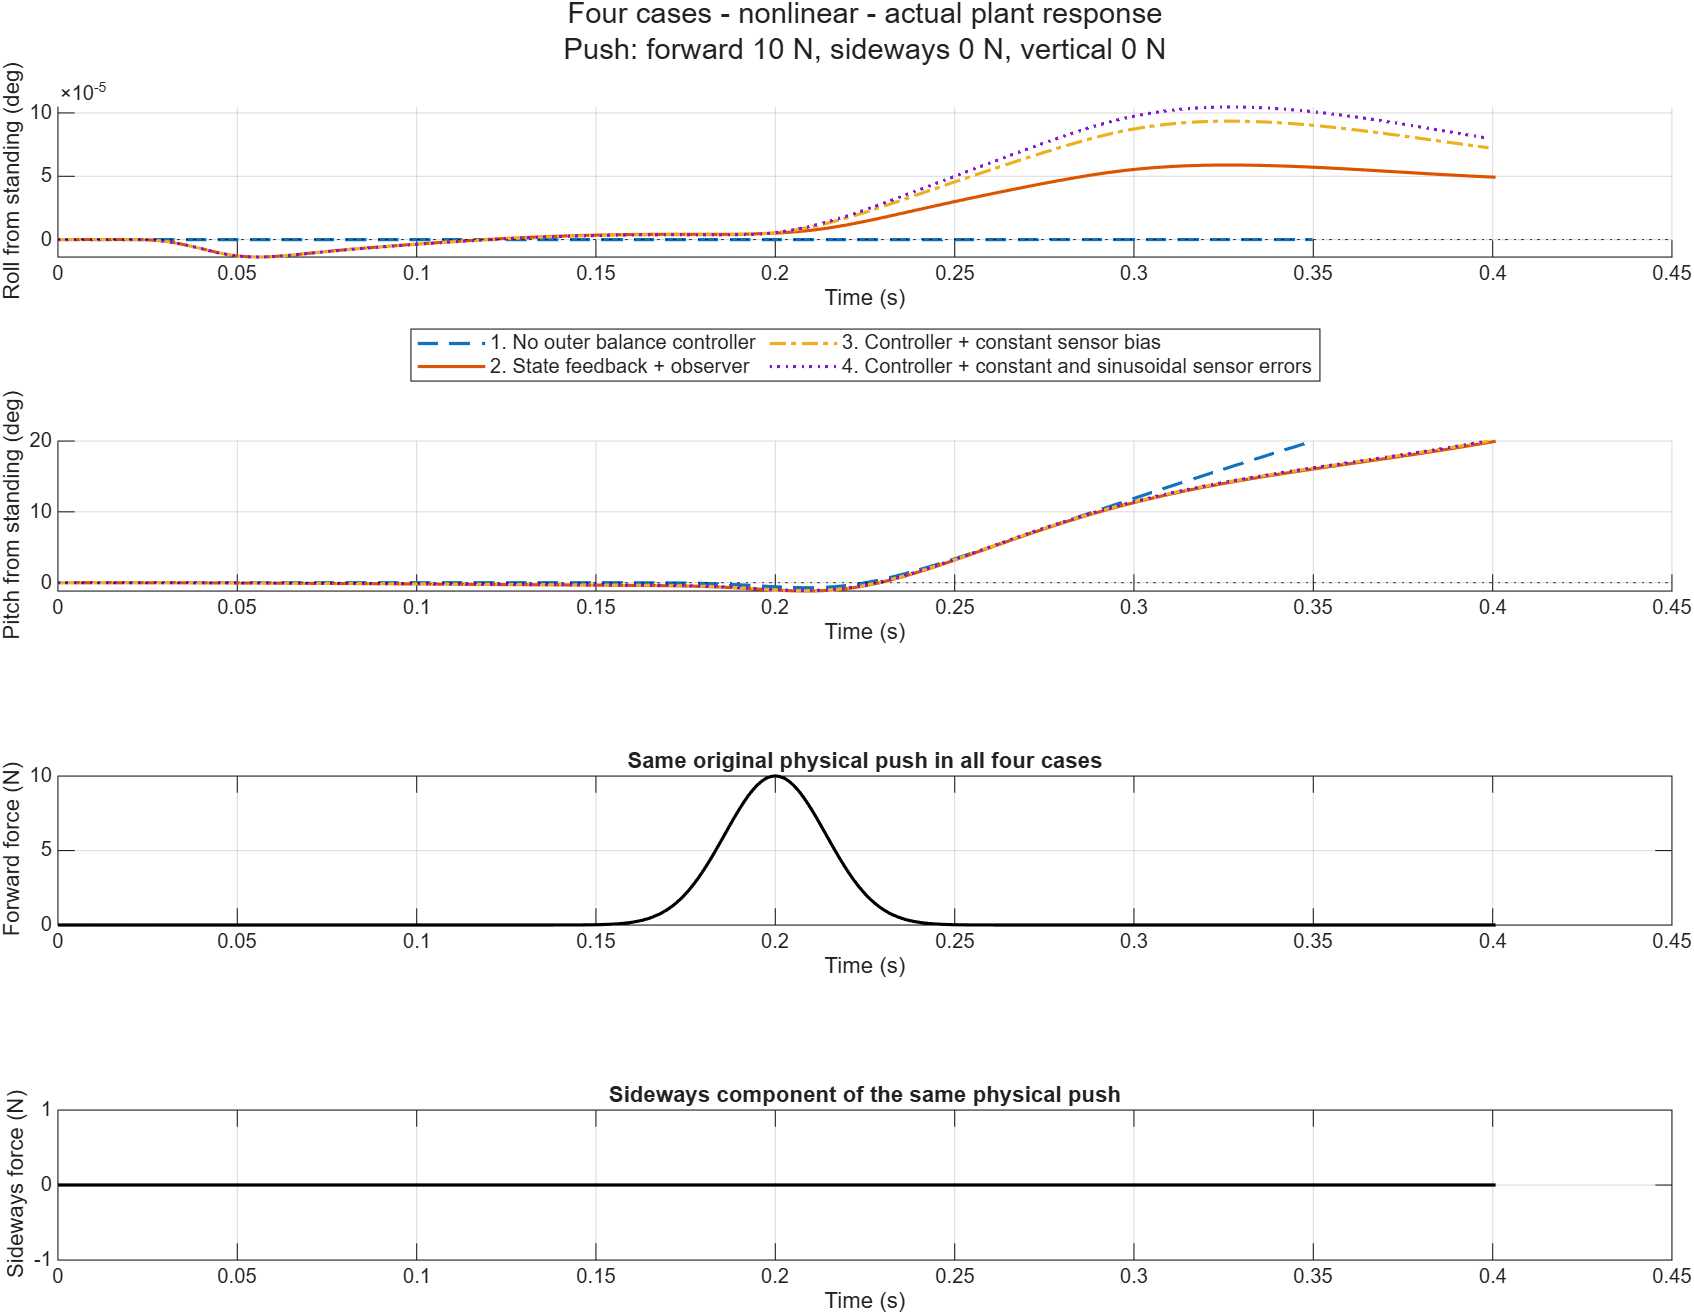
\includegraphics[width=0.485\textwidth]{figures/forward_10N_nonlinear_response.png}
\caption{Nonlinear forward-push responses at 1~N (left) and 10~N (right). All four cases receive the same force within each test. Curves ending early indicate validity termination. The 10~N run does not demonstrate recovery.}\label{fig:forward_validation}
\end{figure*}

\subsection{Sideways Recovery and Cross-Axis Behaviour}
For nonlinear B, increasing the sideways push from 1 to 5 to 10~N increases peak roll from $0.108^\circ$ to $0.855^\circ$ to $3.195^\circ$, and settling time from 0.666 to 0.824 to 1.098~s. Corresponding $t_r$ values are 0.022, 0.041 and 0.124~s, while $t_p$ values are 0.113, 0.161 and 0.314~s. Reverse-excursion ratios are 55.57\%, 51.61\% and 7.23\%. A smaller ratio at 10~N is not evidence of a smaller absolute response; both the peak and recovery time increase.

The linear B model instead predicts nearly proportional peak rolls of $0.107^\circ$, $0.537^\circ$ and $1.074^\circ$, with settling near 0.667~s for all three forces. The nonlinear 10~N roll peak is almost three times the linear prediction, showing that the local approximation understates the large-push response.

At 1~N sideways, A and B have almost identical roll peaks ($0.107^\circ$ and $0.108^\circ$). This is consistent with a naturally damped lateral response and should not be presented as a major improvement caused by outer feedback. Their pitch behaviour differs: A reaches a $3.881^\circ$ pitch excursion, compared with $0.559^\circ$ for B. At 5 and 10~N sideways, nonlinear A stops at 2.188 and 1.828~s as pitch approaches the validity limit, even though roll has largely decayed. B completes both runs; its peak pitch deviations are $0.556^\circ$ and $1.670^\circ$, respectively. Balance must therefore be judged using both axes and run completion, not the directional roll table alone.

\begin{figure*}[!t]\centering
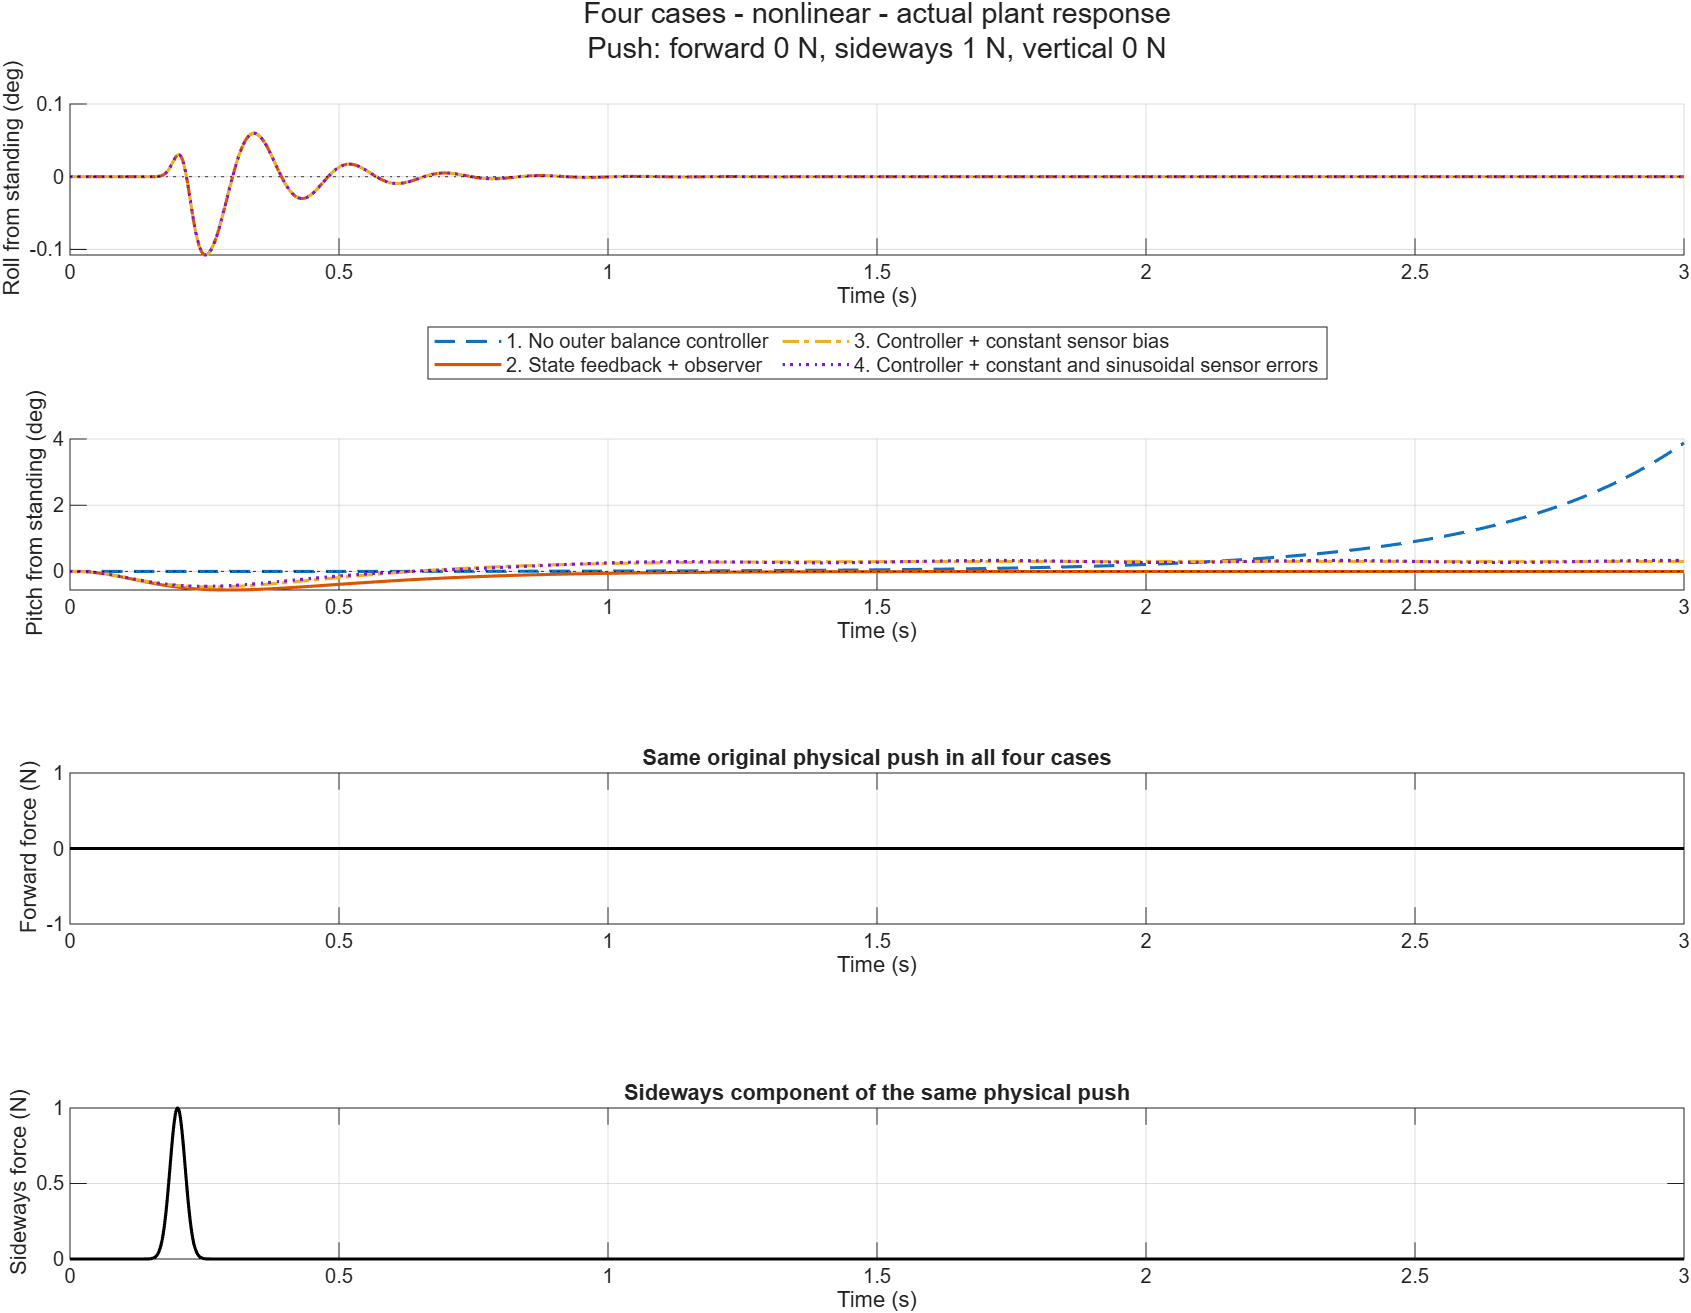
\includegraphics[width=0.485\textwidth]{figures/sideways_1N_nonlinear_response.png}\hfill
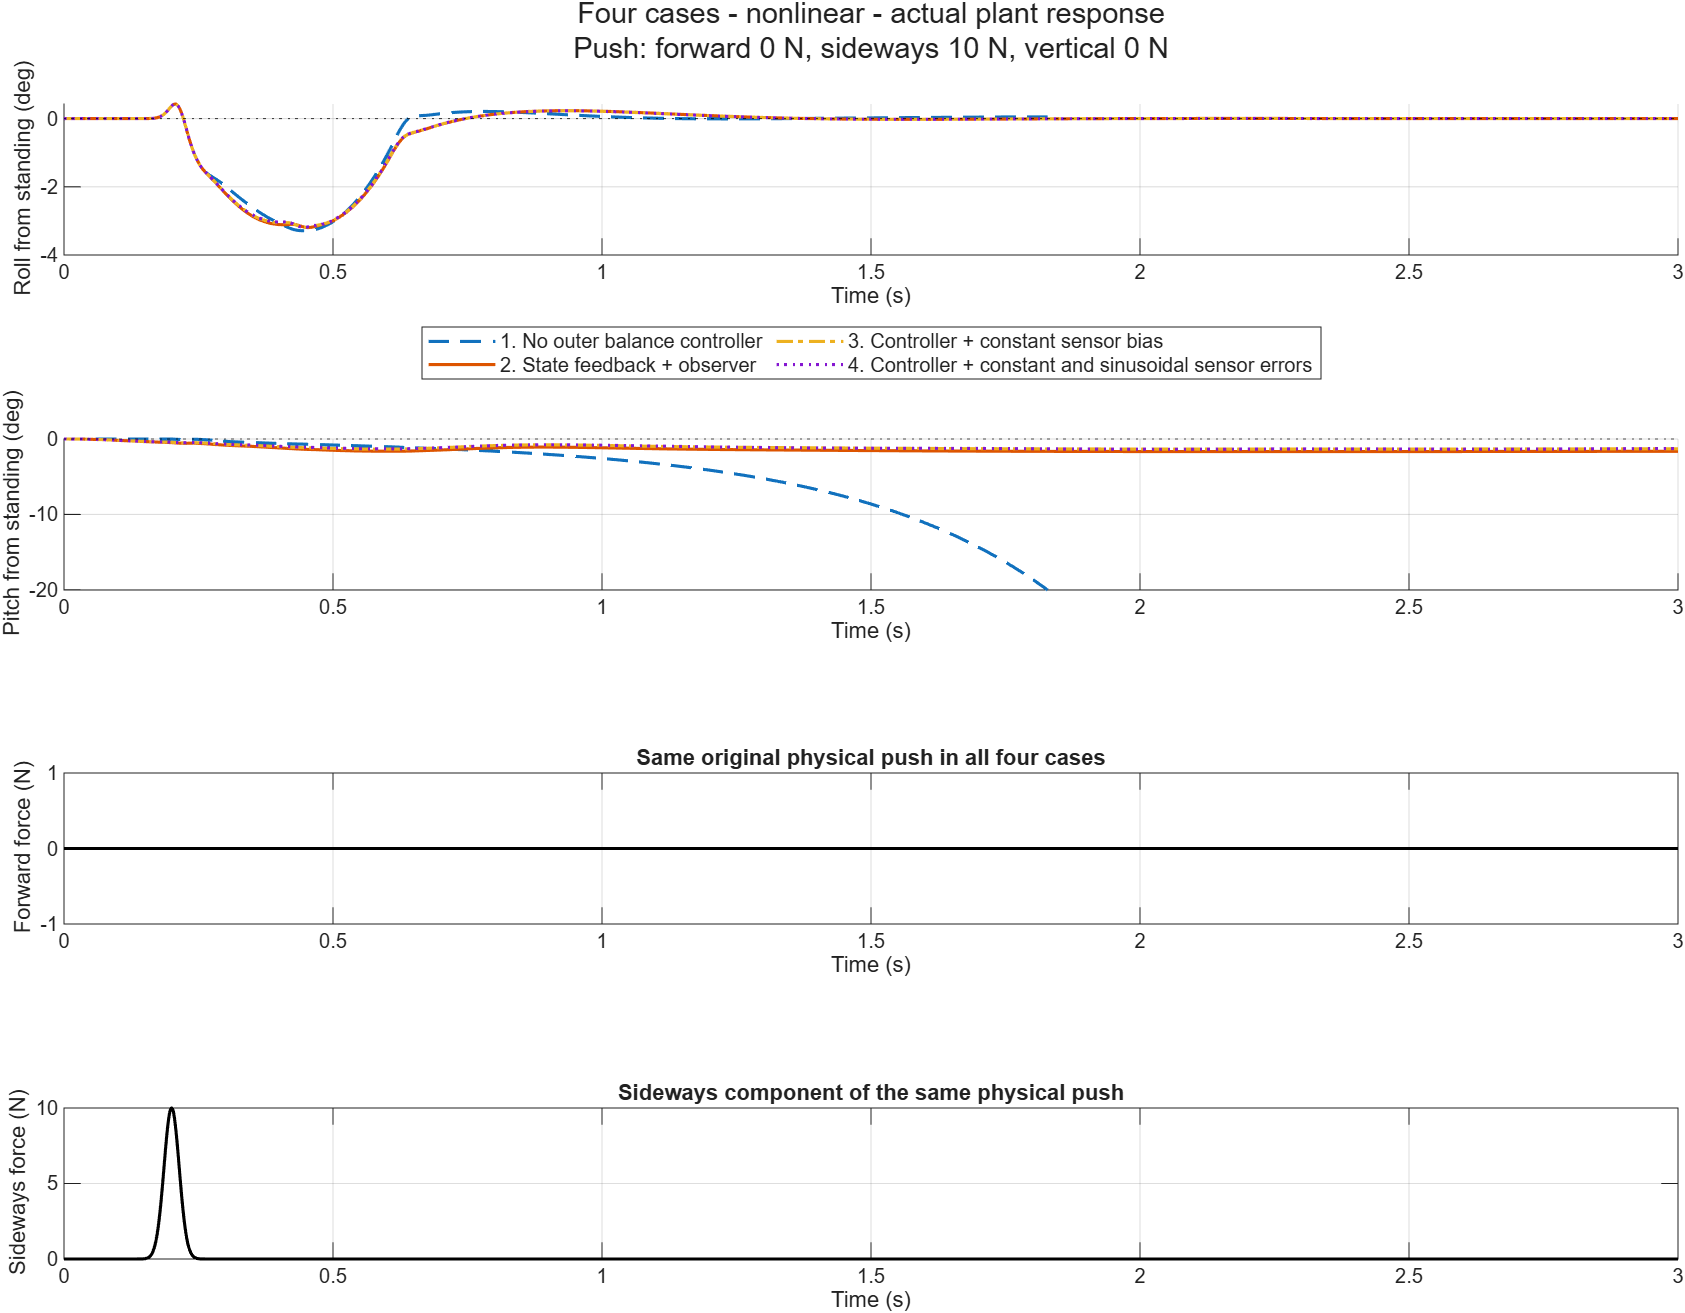
\includegraphics[width=0.485\textwidth]{figures/sideways_10N_nonlinear_response.png}
\caption{Nonlinear sideways-push responses at 1~N (left) and 10~N (right). Similar lateral traces can conceal different pitch stability. Outer feedback prevents the pitch divergence seen in the 10~N inner-servo-only case.}\label{fig:sideways_validation}
\end{figure*}

\subsection{Sensor Errors, Actuation and Scope of Validation}
For the nonlinear 1~N forward test, bias increases peak pitch from $1.474^\circ$ in B to $1.656^\circ$ in C; adding sinusoidal errors raises it to $1.708^\circ$ in D. At 3~s, C and D have pitch deviations of $0.304^\circ$ and $0.333^\circ$. Neither meets its peak-relative 2\% upright settling band. The same residual deviations appear after the 5~N forward push. Thus these sensor errors do not prevent run completion at 1 or 5~N, but they degrade upright regulation. The regulator has no integral or explicit sensor-bias estimation mechanism, so unbiased zero-error recovery cannot be inferred from nominal pole stability.

By contrast, the directional roll metrics change little between B, C and D for sideways pushes. This only establishes low sensitivity of roll to the chosen deterministic error pattern; it does not establish general IMU/encoder noise immunity. In particular, pitch offsets remain visible. Also, the linear 10~N C and D runs receive finite settling times of 1.577 and 1.647~s despite residual pitch near $0.3^\circ$: their large peaks create loose 2\% bands of approximately $0.38^\circ$. A finite peak-relative settling time is therefore not equivalent to satisfying a fixed absolute posture-error requirement.

The eight-motor plots show delivered torques, including the standing holding torque, with the $\pm0.60$~N\,m limits. The displayed nonlinear 5~N forward and 10~N sideways traces remain visibly inside those limits. The failed 10~N forward case also ends without delivered torque visibly reaching the cap. This does not prove that requested angle corrections were unclipped: the outer $\pm8^\circ$ correction limit, absolute joint-target limits and actuator lag must be assessed separately. The MAT summary contains no torque maxima, clipping durations or contact-load histories; consequently it cannot establish numerical torque margins or absence of foot lift.

\begin{figure*}[!t]\centering
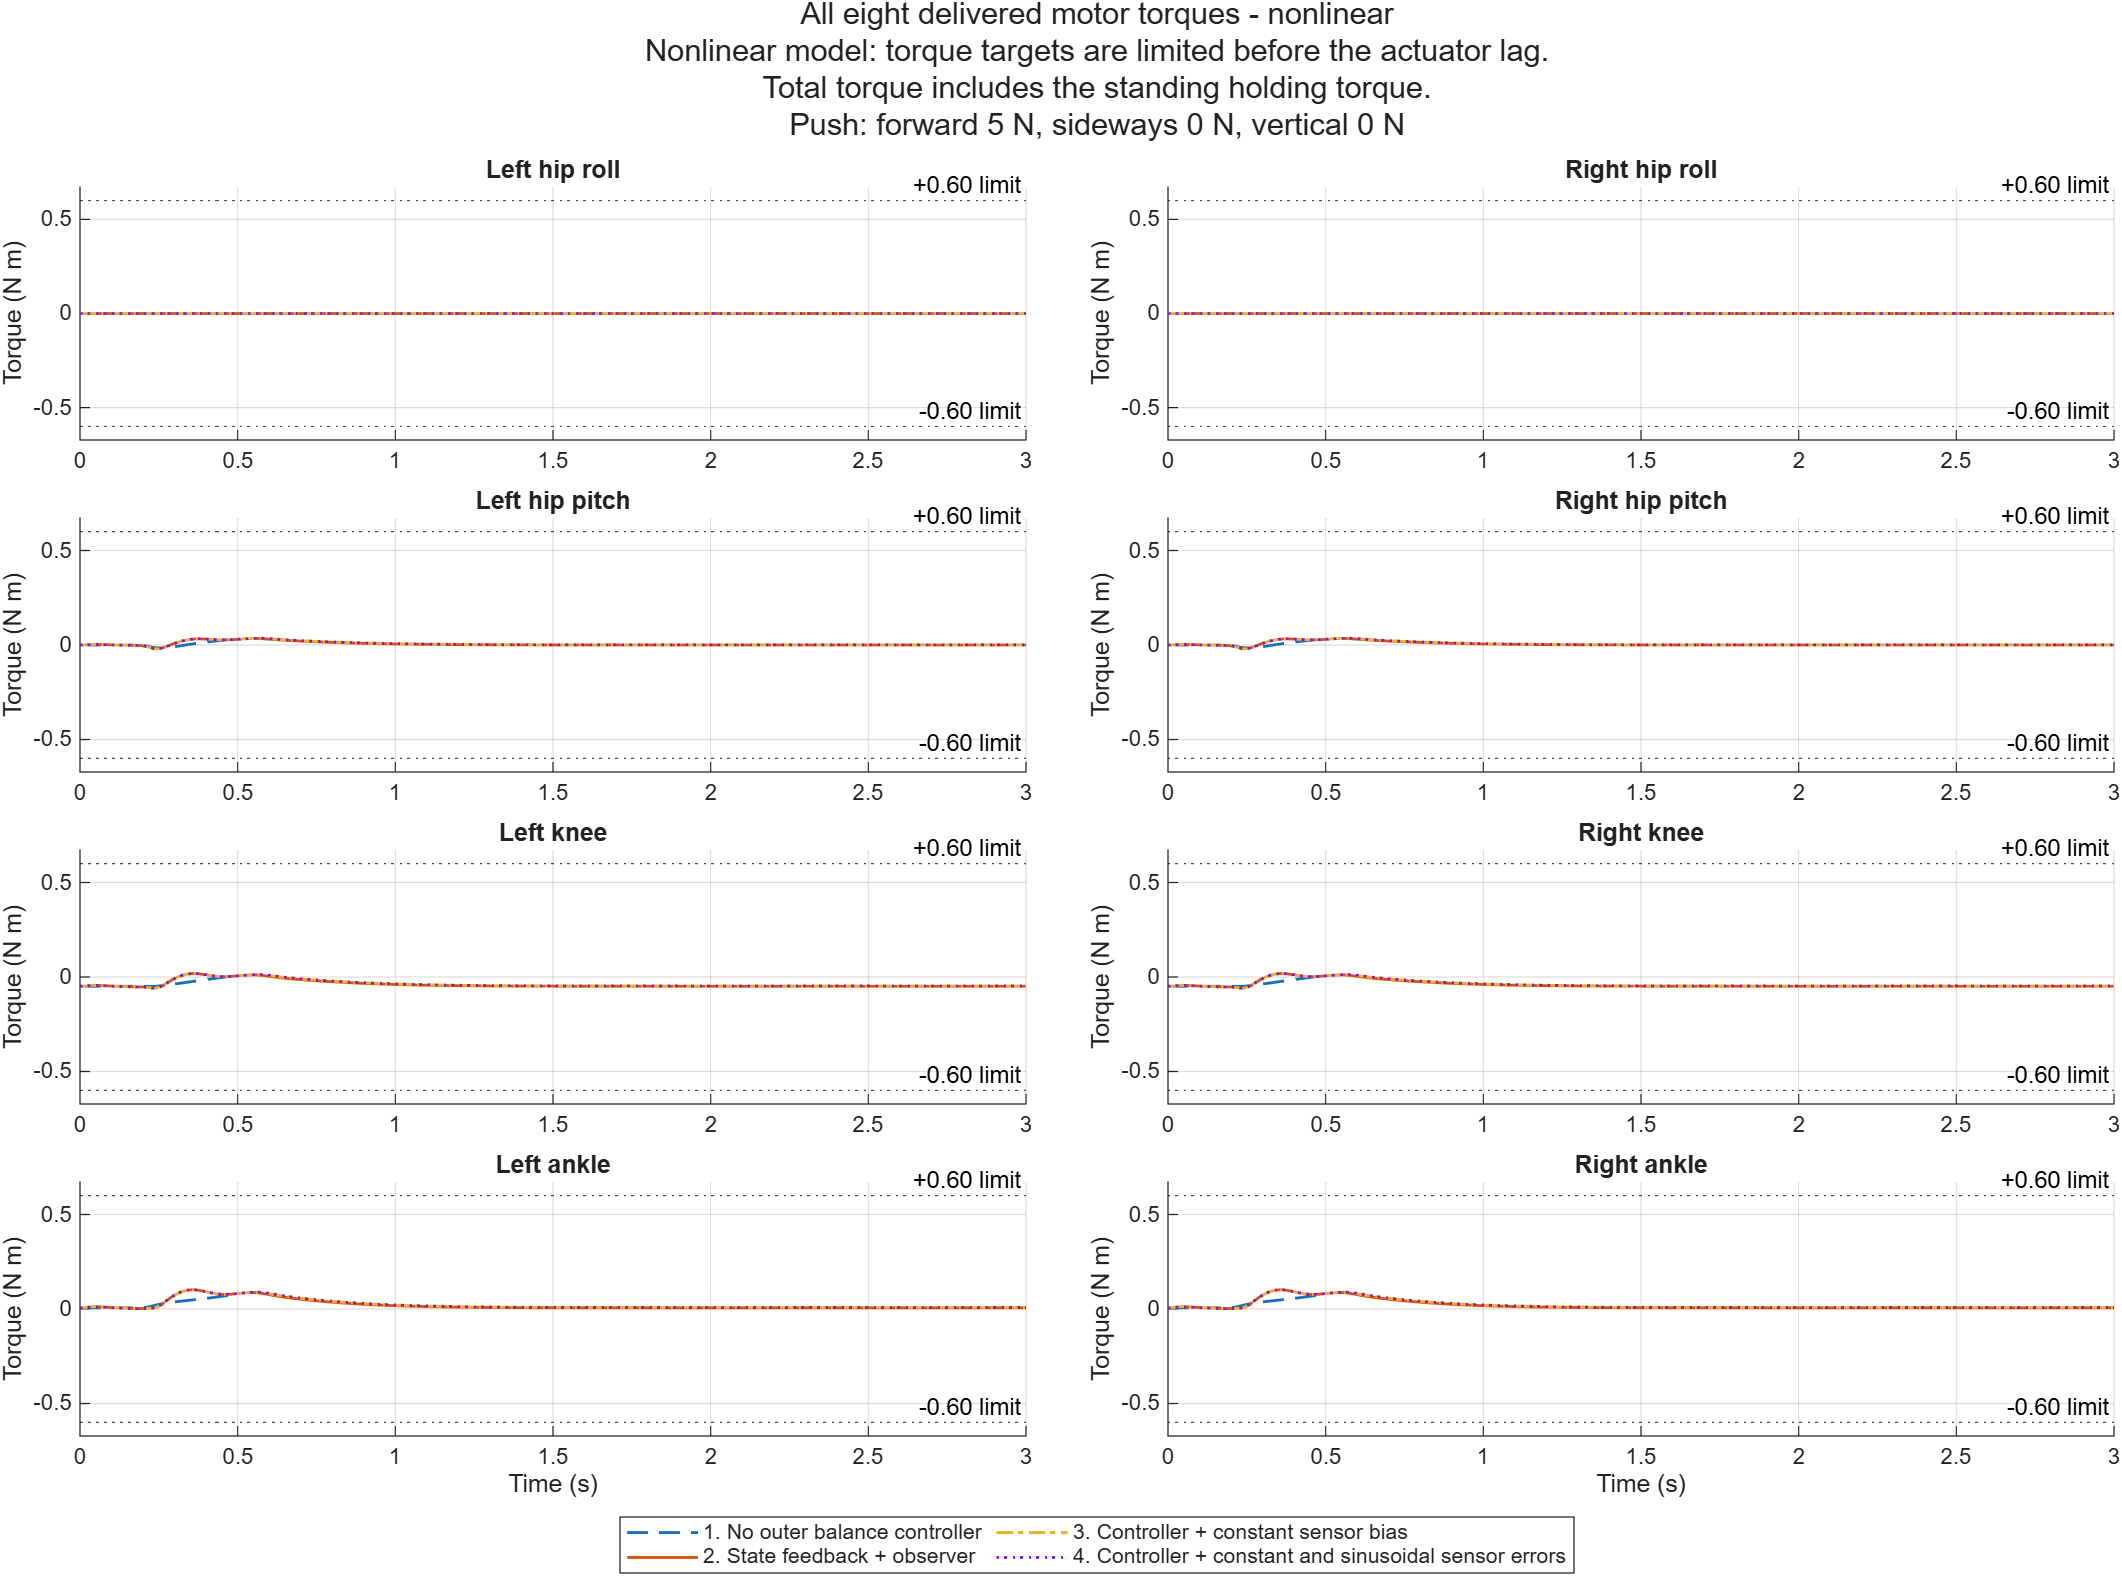
\includegraphics[width=0.485\textwidth]{figures/forward_5N_nonlinear_torques.png}\hfill
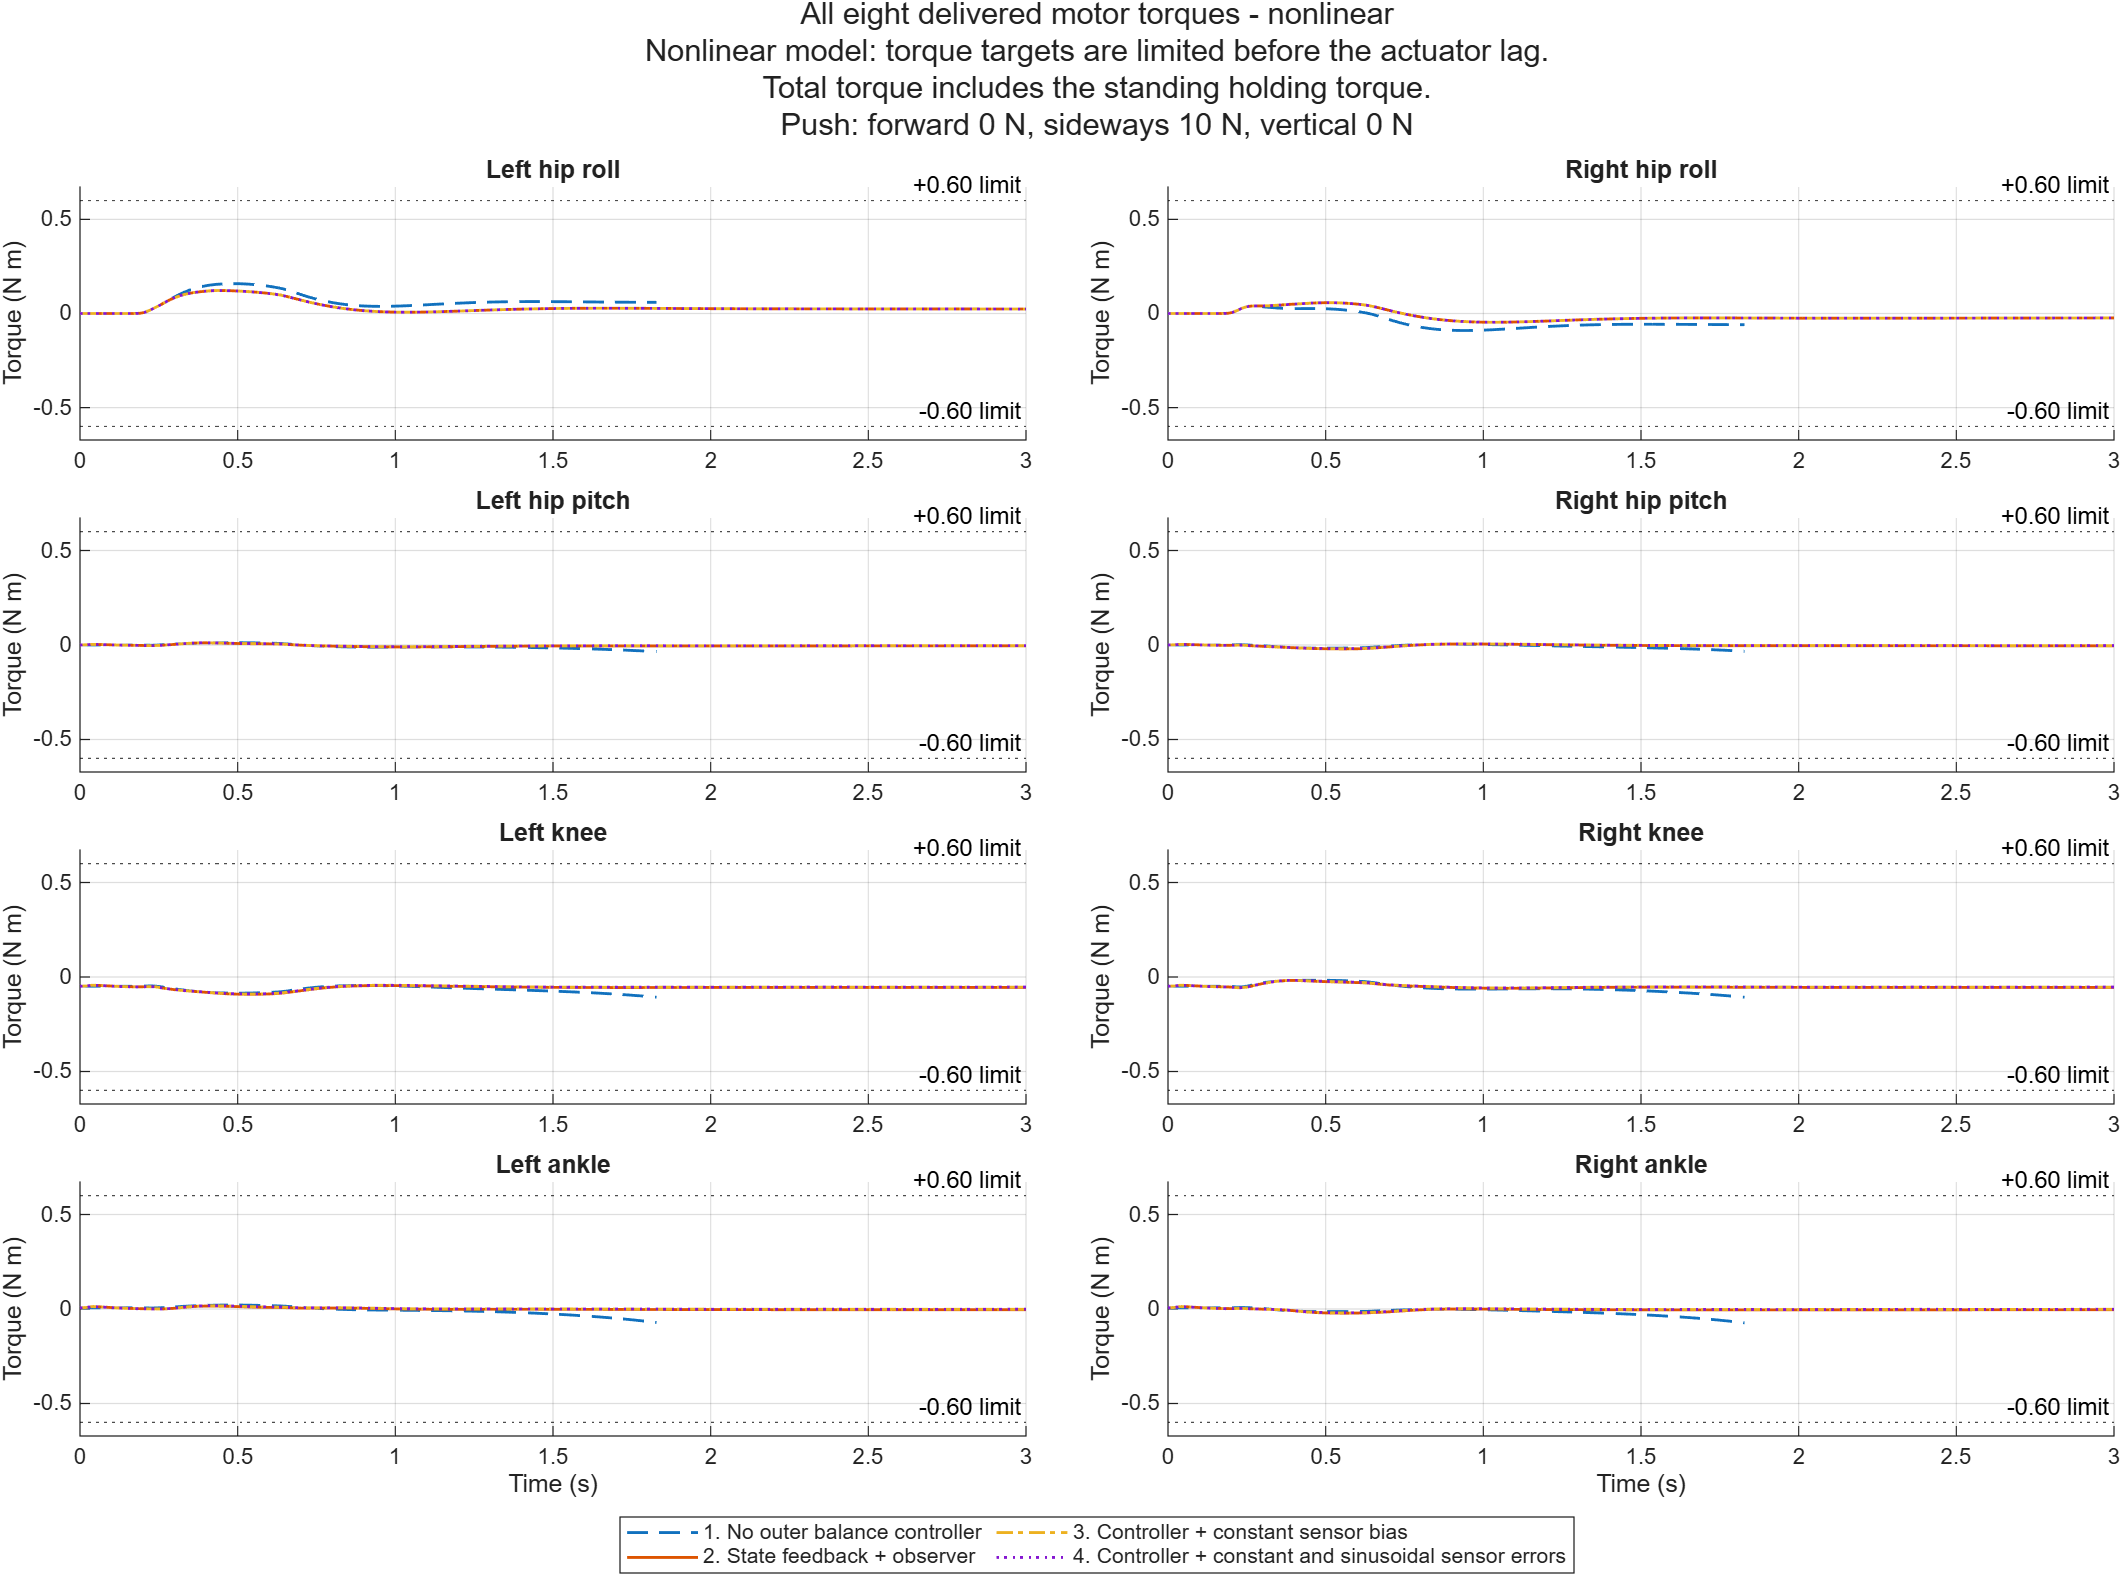
\includegraphics[width=0.485\textwidth]{figures/sideways_10N_nonlinear_torques.png}
\caption{Delivered torque for all eight motors during the nonlinear 5~N forward and 10~N sideways tests. The dotted lines indicate the motor torque caps. Torque remaining below the cap does not establish that command limits or support constraints are inactive.}\label{fig:torque_validation}
\end{figure*}

These experiments demonstrate nominal observer-based push recovery within the tested range, with clear direction-dependent limitations. The $5^\circ$ roll/pitch bound is respected in the controlled nonlinear 1~N forward and all three sideways tests, but is violated in the 5~N forward test; the 10~N forward test terminates. Settling after a push does not validate the separate $2^\circ$ initial-tilt requirement. The saved results also do not establish observer-error convergence time, uncertainty-grid robustness with fixed gains, gain/phase margins, lean-reference tracking, constant external-moment rejection, delay/backlash robustness or stochastic-noise torque statistics. These require dedicated measurements or experiments. No PID ranking, hardware-performance claim or complete satisfaction of the design criteria follows from the present batch.
